\section{XHC WHB04 Pendant/MPG} 

EazyCNC supports a commercially available MPG named WHB04, 
see Figure~\ref{fig:whb04}. This is a wireless model, a 
sister model called HB04 with wired USB connection is also available 
and it is supposed to be 100\% compatible but this has not been tested.

The WHB04 pendant is not particularly excellent, the wheel sometimes misses
pulses, the display update speed is nothing to write home about and the
wireless link exhibits a glitch every now and then. But it is what
we have at the moment.

Note worthy is also that WHB04 has a battery saving mode that kicks in
in a about thirty seconds and stops the display from updating unless
you wake the pendant up by pressing a button, turning a knob or moving the wheel.

Having said all that, it is still a useful device.

\begin{figure}[htb]
    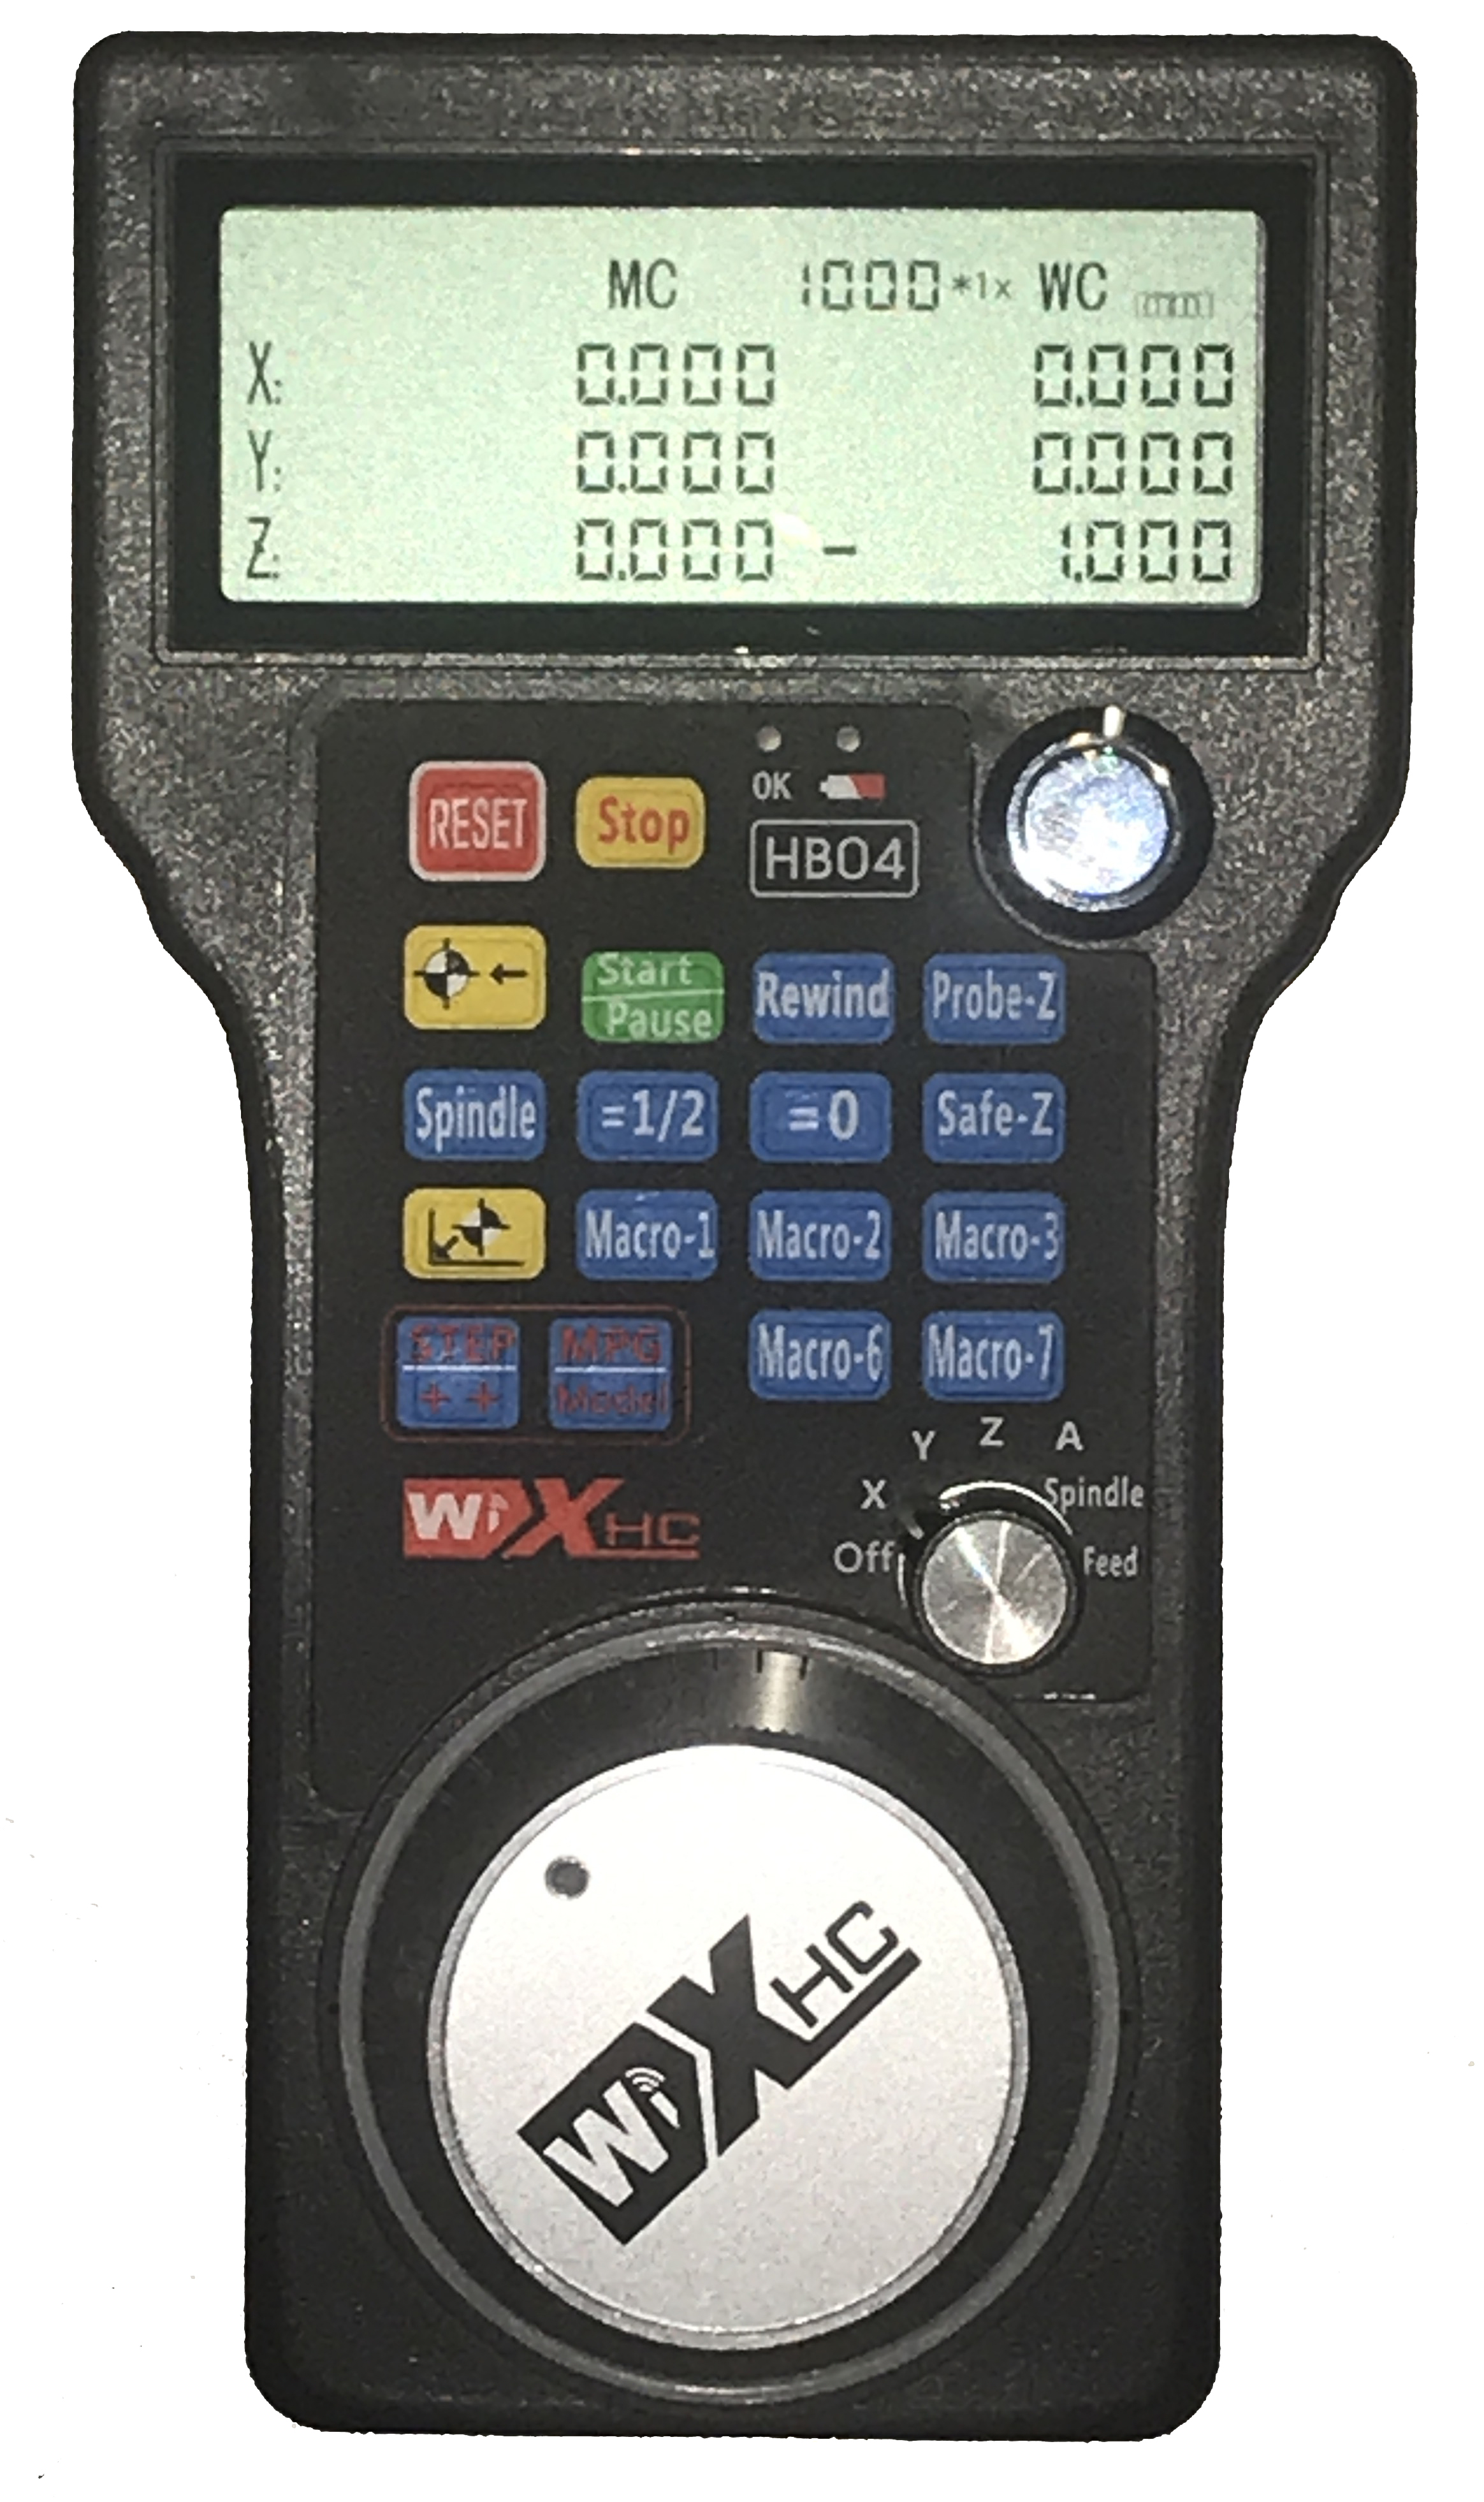
\includegraphics[scale=0.05]{whb04.jpg}
    \caption{WHB04 Pendant/MPG  }
    \label{fig:whb04}
    \end{figure}

 

\subsection{WHB04 Controls}

Figure~\ref{fig:whb04-keypad} shows a close up of the WHB keypad.

The two main controls of the MPG are the small axis selector knob  you can see in the closeup 
and the large pulse wheel.

In general the axis selector selects which axis or other parameter is affected
by the pulse wheel or buttons on the keypad. 
 
For some functions setting the selector knob to 'Off' will make those functions
apply to all axes at once.

\begin{figure}[htb]
    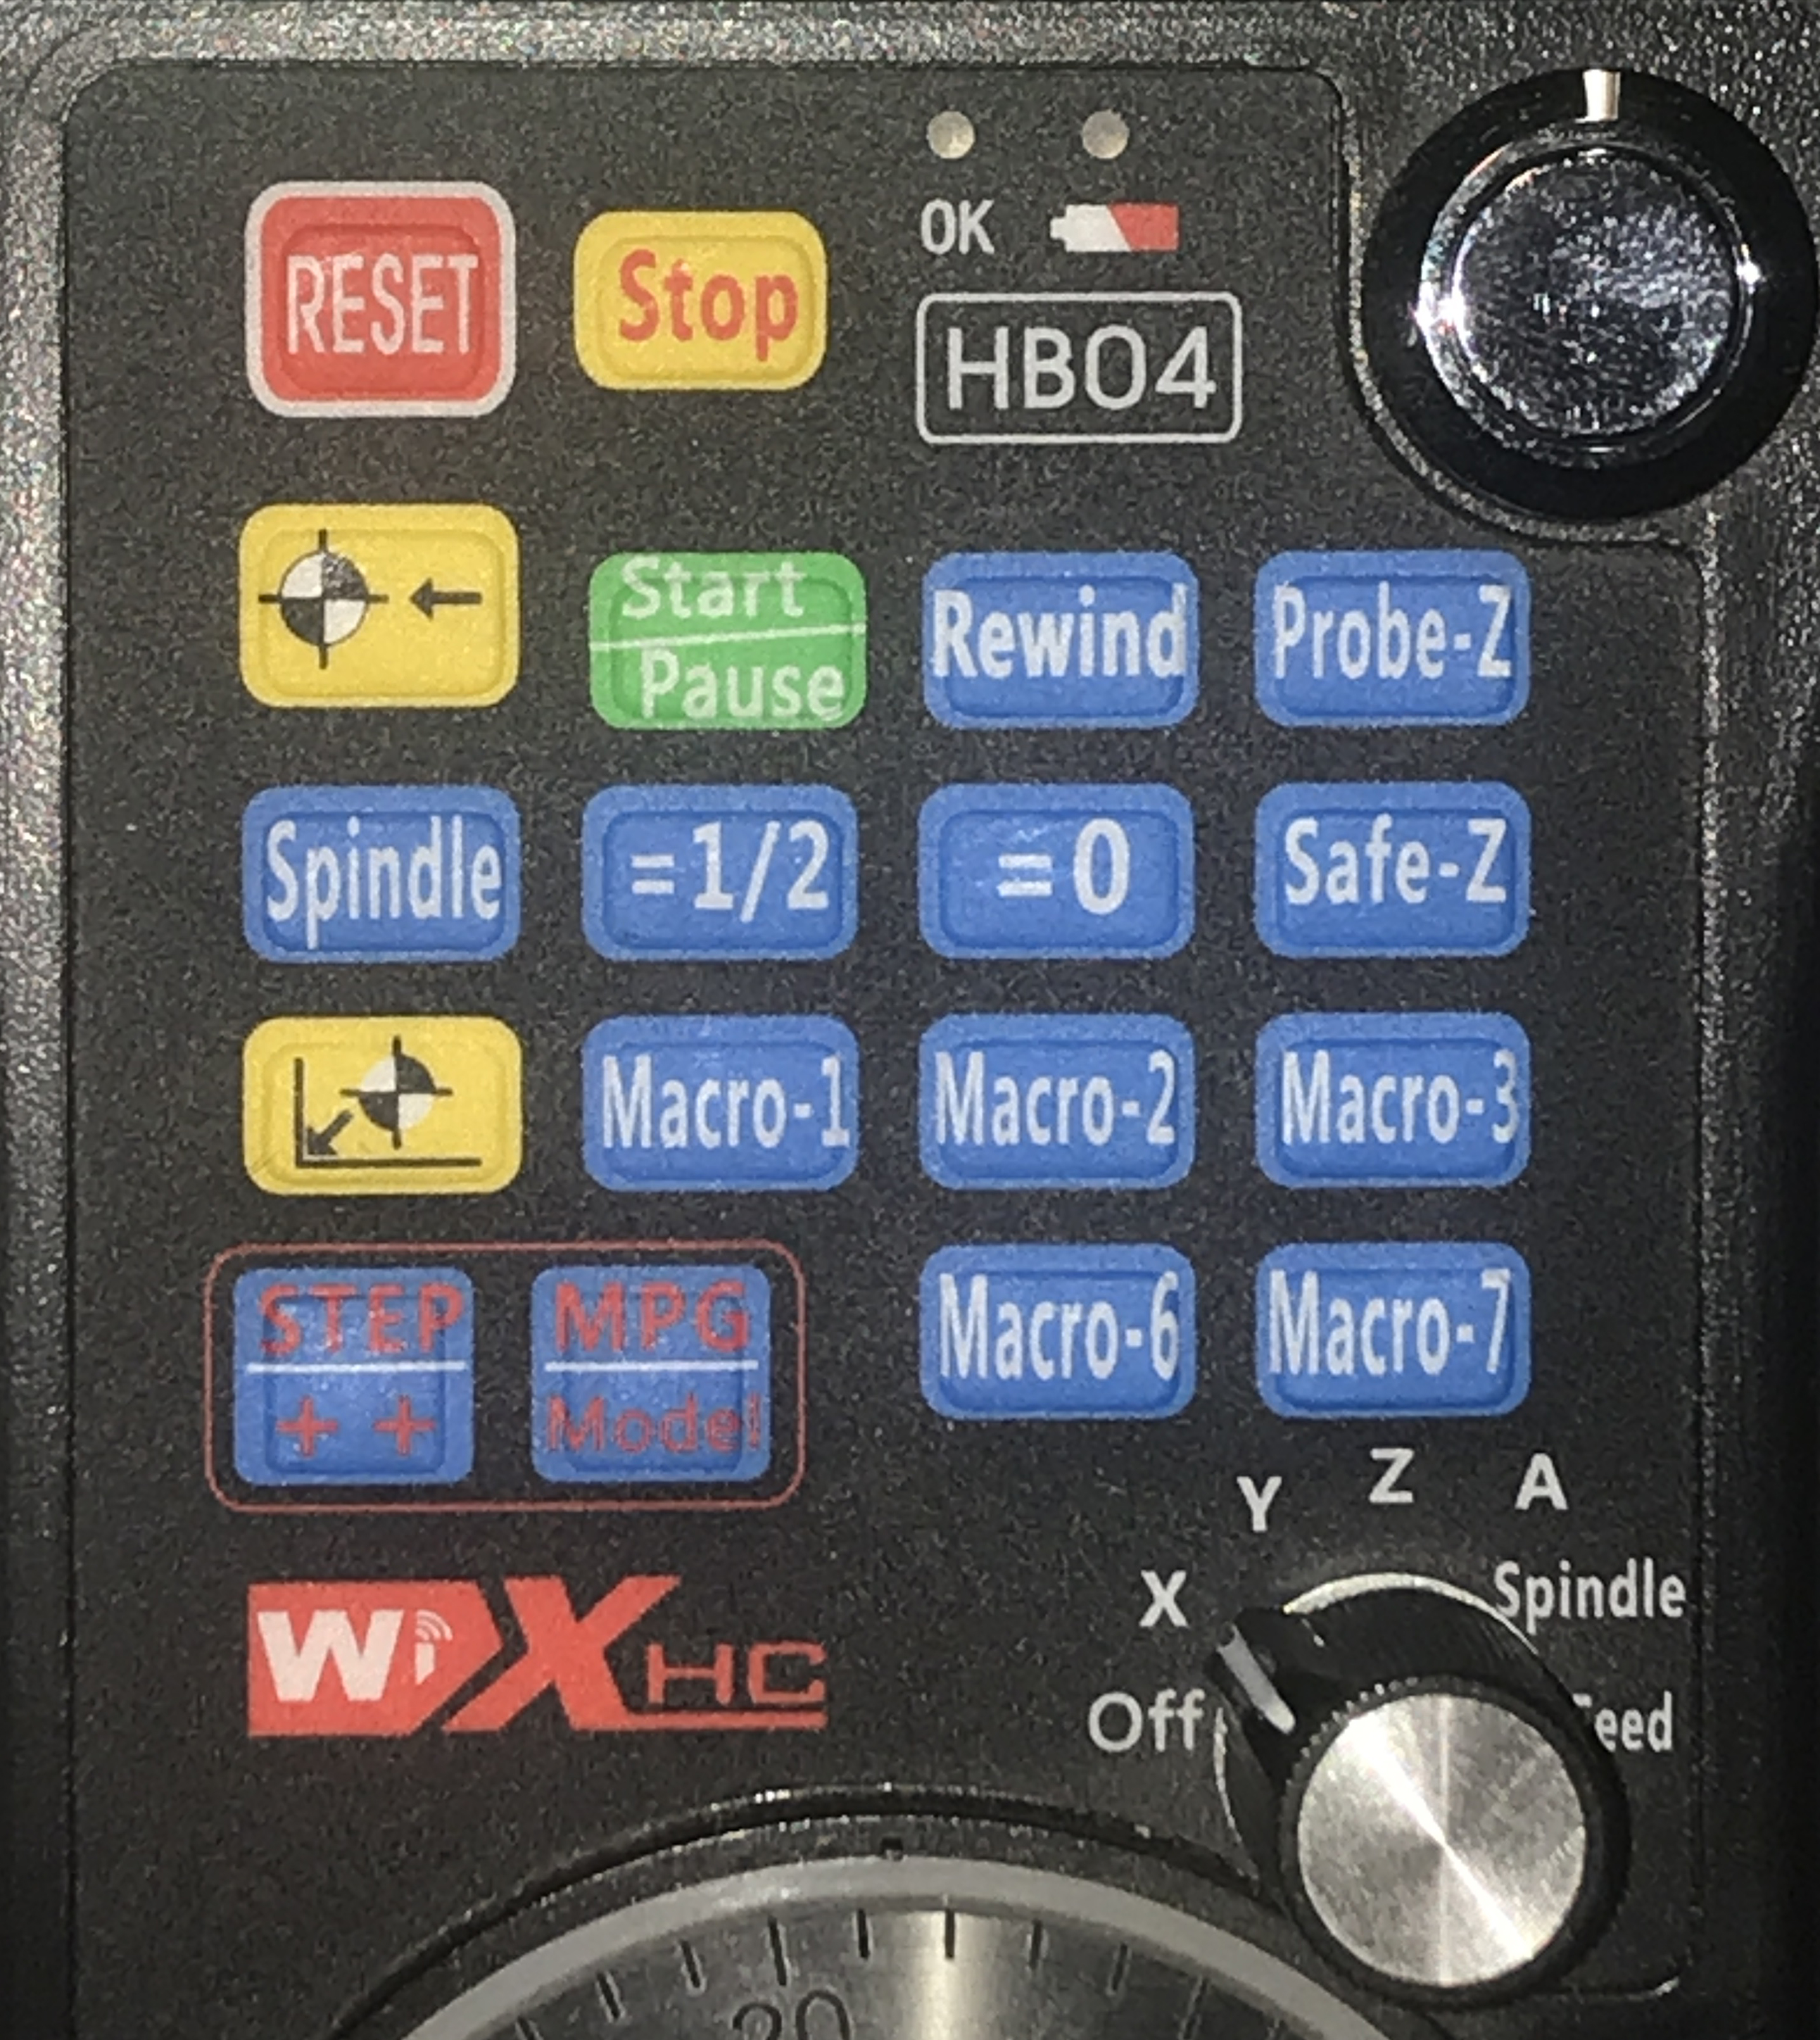
\includegraphics[scale=0.10]{whb04-keypad.jpg}
    \caption{WHB03 Keypad}
    \label{fig:whb04-keypad}
    \end{figure}


\subsection{WHB04 Display}

Figure~\ref{fig:whb04-display} shows a close up of the WHB04 display.

The display has DROs for three axes at a time. If the axis selector
is in X,Y or Z position then the corresponding axis values are 
displayed in the DROs. If the selector is in A position then axis positions
of the A, B and C axis are displayed.

The DROs in the 'MC' column are not used (to avoid confusion) and always display'0.000'

The DROs in the 'WC' column display the same DRO values as on the EazyCNC computer screen.

Note that you can NOT see more decimals on the pendant DRO than on the computer screen 
eventhough the pendant always displays three digits.

Next to the WC text to the right an 'inch' or 'mm' sign is show and reflects 
weather the DRO values and wheel operate in inch or mm mode. This is controlled
by the units selected for the DROs in EazyCNC.
   
%---------------------------------------------------------------------------
\begin{figure}[htb]
    \includegraphics[scale=0.]{whb04-display.jpg}
    \caption{WHB04 Display }
    \label{fig:whb04-display}
    \end{figure}

\subsection{WHB04 Wheel}


Every 'click' of the wheel moves the selected axis one step to the wheel direction.
The speed at which the mill table,head or plasma torch moves is relative to how fast you
turn the wheel. 

In principle the wheel allows absolute (well incremental really) control of 
the axis position and speed. In practice the wheel sometimes misses pulses 
so turning the wheel ten clicks may only result in nine steps, always
confirm by looking at the DROs.

Because it is possible to turn the wheel faster than the axis can move there
is a windup prevention that prevents the wheel position from advancing too 
much beyond where the axis has advanced.

Because of the long chain of hardware and software that connects the pulse wheel
to the axis stepper motor, the feel of control you get with the wheel is far from 
perfect. However it does allow you to control the axis position rather
swiftly and accurately.

The 'step size' i.e. how much every wheel click moves milling table is displayed
to the left of the 'WC' text. It is expressed as number of 1/1000th of the 
units selected for the DROs. Very much like the jogging step selection but 
separate from that.

In 'mm' mode the displayed text and step size are as follows:

\begin{tabular}{ r | l }
x1000 &  1.000 mm \\
x100  &  0.100 mm \\
x10  &   0.010 mm \\
x0   &   1 stepper step \\
\end{tabular}

In 'inch' mode the displayed text and step size are as follows:

\begin{tabular}{ r | l }
x100  & 0.100 inch \\
x10   & 0.010 inch \\
x1    & 0.001 inch \\
x0   &   1 stepper step \\
\end{tabular}

You change the step size with the 'STEP++' key, see below.

\seticons{whb04-step-button}
\subsection{Step++ -key}       
   
Pressing this key shortly will advance the step size to the next \emph{smaller}
size. After 'x0' the step size reverts to the largest steps size ('x1000'
for 'mm mode and 'x100' for 'inch' mode).

A long press (over 1 seconds) will revert the step size tolargest steps size.

Whenever the largest step size is selected a long 'beep' sound is emitted
from the computer to alert the user.

\seticons{whb04-auto-touch-xy-button}
\subsection{Probe XY -key}  


Pressing this key has the same effect as 
pressing the -X or -Y Touch button in the Work Offsets screen when the 
'Use PROBE to Touch' feature is enabled.

In other word this will perform a short probing move on the selected 
axis and as soon as the probe trips the movement stops and rectracts 
and the selected axis work offset is set to the negative half value of 
the Probe Diameter parameter in 
the Work Offsets screen.

Thus this is a handy way to perform edge finding using a probe and the MPG.

Use the axis selector knog to select either X or Y axis. You can only
probe on the left/front side of the work piece with this key.

\seticons{whb04-probe-z-button}
\subsection{'Probe Z' -key}       
 
Pressing this key has the same effect as 
pressing the Touch button in the Work Offsets / Set Z origin screen when the 
'Use PROBE to Touch' feature is enabled.
    
In other word this will perform a short probing move on the Z axis 
axis and as soon as the probe trips the movement stops and rectracts 
and the Z axis work offset is set to the Gage Height parameter in 
the Work Offsets screen.
    
Thus this is a handy way to perform 'zero' the Z-axis with the probe.
    

\seticons{whb04-spindle-button}
\subsection{Spindle -key}  

Pressing this key has the same effect as pressing the SPINDLE button on 
the computer screen. 

In other words it toggles the spindle on and off.

\seticons{whb04-start-pause-button}
\subsection{Start/Pause -key}  

This key has the same effect as pressing alternatively the RUN and HOLD buttons
on the computer screen.

\seticons{whb04-stop-button}
\subsection{Stop -Key}       

This key has the same effect as pressing the STOP button on the computer screen.
 
\seticons{whb04-half-button}
\subsection{'=1/2' -key}       

Pressing this key has the same effect as 
pressing the Touch -X or Touch -Y  button in the Work Offsets screen when the 
'Use PROBE to Touch' feature is NOT enabled.
    
In other words the selected axis Work Offset is set to the negative half value of the Probe Diameter parameter in 
the Work Offsets screen.
    
Thus this is a handy way to perform edge finding manually with 
an edge finder and the MPG.
    
Use the axis selector knog to select either X or Y axis. You can only
Touch on the left/front side of the work piece with this key.
            
\seticons{whb04-goto-origin-button}     
\subsection{'Goto Origin' -key}       
       
Pressing this key will cause the X and Y axis to jog to the zero
position of the DROs.


\seticons{whb04-zero-button}     
\subsection{'=0' -key}       

Pressing this key has the same effect as 
pressing the ZERO button in the selected axis.

Use the axis selector knob to select the affected axis, or set the
axis selector knob to 'Off' to ZERO all axis.

\seticons{whb04-safe-z-button}          
\subsection{Safe Z -key}       

                                              
Pressing this key will cause the Z-axis to move to the 
Safe Z value set in the Axis Setup / Axis Z.

\seticons{whb04-reset-button}
\subsection{Reset -key}       

                                              
Pressing this has the same effect as pressing HOME button on the computer 
screen.

Use the axis selector knob to select the affected axis, or set the
axis selector knob to 'Off' to HOME ALL axis.

A long press will force HOME ALL action regardless of the axis selector knob position.


\seticons{whb04-rewind-button}
\subsection{Rewind -key}       

Pressing this key will change the currently selected tool to the next tool number, 
in other words this has the same effect as L-word in G-code. Note that it does
not actually cause any tool change but does effect the tool offset, if it is 
enabled with G43 code.

Long press will reset the current tool to tool number 1. 

Whenever the tool number1 is selected  a long 'beep' sound is emitted
from the computer to alert the user.

This key is mainly intended to help setting up tool length without touching
the computer keyboard.






\newcommand{\noicons}{\savebox{\iconbox}{}}
\noicons

